\chapter{Implementation}\label{ch:Implementation}

\section{Exploratory Data Analysis}
All code for the EDA detailed in this chapter can be found at:\newline https://github.com/AMacleod79/HonoursProjectCode
\subsection{Data Overview}
\subsubsection{Cervical cancer dataset}
The cervical cancer dataset was obtained from kaggle.com. \newline
(see https://www.kaggle.com/loveall/cervical-cancer-risk-classification)\newline
This dataset does not look at predicting if someone will or will not have cervical cancer, however it looks at attributing a risk factor for cervical cancer or not. Cervical cancer is a complicated diagnostic to make and as such there is not one single test to confirm diagnostic. The positive risk factor is inferred from the combination of the last four column: Hinselmann, Schiller, Citology, Biopsy \cite{Fernandes:2017td} (also cite the discussion page on kaggle).
The dataset contains 858 instances with 32 features and 4 target variables for each of the test carried out.
The exploratory data analysis carried out on this dataset can be found in the cited github repository as CervicalCancerEDA.R.
The 32 features focus on lifestyle factors previously shown to influence cervical cancer risk in women, namely:
%need to list the attributes here
An examination of the data structure showed that 27 columns were factors, with the column "smoke pack per year" showing 63 levels. The Random Forest function in R will only handle a maximum of 53 levels and therefore the data in this column needed to be manipulated to accommodate this restriction. First any missing values was replaced by the mean for the column. Then it was found that there were a high number of discrete values between 0 and 1 for the number of pack of cigarettes smoked per year, and these were all considered as independent levels. All values that were less than 1 for this column were replaced by 0, taking the total number of levels for the column from 63 to 42, which is now manageable by Random Forest.
All the other columns had a number of factor levels smaller than 53 and were left as such, however any missing value was replaced by the mean for the column in which it was found.
A composite target variable calculated as a mean value of all 4 target variables (Hinselmann, Schiller, Citology, Biopsy was created and added as the last column in the dataset (rounded to 0 or 1).
Finally the class distribution was represented as a bar chart (see Figure 4.1) and the modified dataset was exported as a new csv file to be used in the later stages of this projects.

\begin{figure}[H]
    \centering
    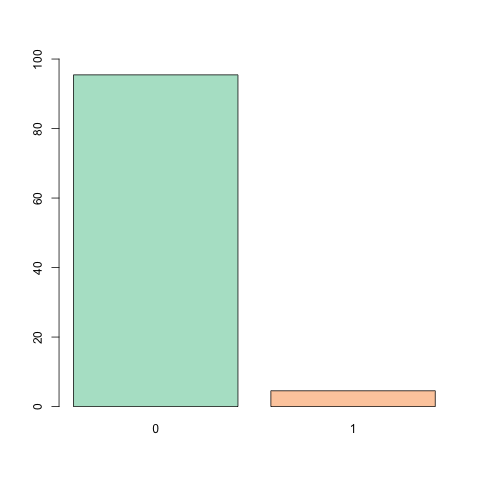
\includegraphics[width=0.8\textwidth]{ThesisTemplate/usingLatex/chapter4Images/figure4_10.png}
    \caption{Class Distribution of cervical cancer dataset.\newline
    0 represents the absence of cervical cancer risk for an individual and 1 represent the presence of cervical cancer risk.}
    \label{fig:my_label}
\end{figure}


\subsubsection{Breast cancer dataset}
This dataset was obtained from kaggle.com. \newline
(see https://www.kaggle.com/uciml/breast-cancer-wisconsin-data) \newline
This dataset was developed with a view to train and test algorithms to determine whether a breast tumour was malignant or benign \cite{}. \newline
% need citation here
The dataset is comprised of 569 instances each with 32 attribute and one target label (B for benign and m for malignant).\newline
The attributes were computed from images of a fine needdle aspirate of a breast mass to describe the characteristics of the cell nuclei present in the image. The features were as follows:
\begin{itemize}
    \item radius (mean of distances from center to points on the perimeter)
    \item texture (standard deviation of gray-scale values) 
    \item perimeter 
    \item area 
    \item smoothness (local variation in radius lengths) 
    \item compactness (perimeter\^2 / area - 1.0)
    \item concavity (severity of concave portions of the contour)
    \item concave points (number of concave portions of the contour)
    \item symmetry
    \item fractal dimension ("coastline approximation" - 1)
\end{itemize}
The mean, standard error and mean of of three largest values (i.e. the "worst") for each of the feature was calculated and documented as a feature for each image.\newline

The exploratory data analysis carried out on this dataset is documented in the cited github repository as BreastCancerEDA.R.\newline
An analysis of the data structure showed no missing values. The target variable was expressed as B or M and was recoded to be either 0 (begign) or 1 (malignant), further the target variable was originally the second column but for ease of analysis in the next stages of the project this was moved to be the last column and renamed "Label".
Finally the class distribution of the dataset was computed and is shown in figure 4.2 and the modified dataset was exported as a csv file for later use in the project.

\begin{figure}[H]
    \centering
    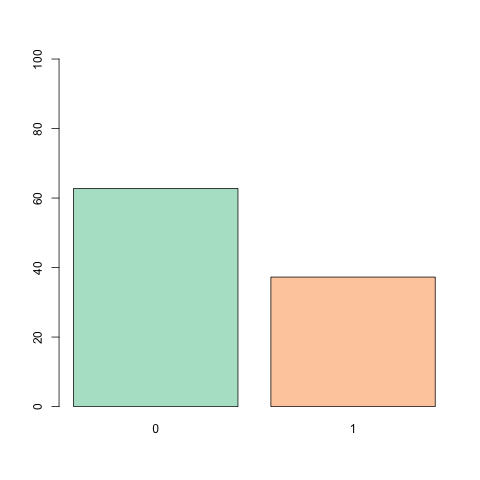
\includegraphics[width=0.8\textwidth]{ThesisTemplate/usingLatex/chapter4Images/figure4_4.png}
    \caption{Class Distribution of the breast cancer dataset.\newline 0 represents the cases were the breast mass was benign and 1 those cases were the mass was malignant.}
    \label{fig:my_label}
\end{figure}

\subsubsection{Liver Disease dataset}

This dataset was obtained from kaggle.com.\newline
(see https://www.kaggle.com/jeevannagaraj/indian-liver-patient-dataset). \newline
%citation needed here
This dataset is made up of 583 instances of patient records with 10 attributes and one target variable to determine whether the patient is a liver patient or not. The attributes are various biochemical measures of liver health as well as patient specific information such as age and gender:
\begin{itemize}
    \item Age of patient
    \item Gender of patient
    \item Total Bilirubin
    \item Direct Bilirubin
    \item Alkaline Phosphatase
    \item Alamine Amino-transferase (sgpt)
    \item Aspartate Amino-transferase (sgot)
    \item Total Proteins
    \item Albumin
    \item Albumin and Globulin Ratio
    \item is patient (target label)
\end{itemize}

The exploratory data analysis carried out on this dataset is documented in the cited github repository as LiverDataEDA.R.\newline
The target label was set to 1 (not a liver patient) and 2 (liver patient), for consistency with respect to the other dataset used in this project, the data was recoded to 0 (not a liver patient) and 1 (liver patient).\newline
A check for missing data revealed only four instances missing a value in the albumin and globulin ratio. The missing values were replaced with the mean for that column.
The class distribution was compiled and presented as a graph (see figure 4.3) and the modified dataset was exported as a csv file for later use in the project.

\begin{figure}[H]
    \centering
    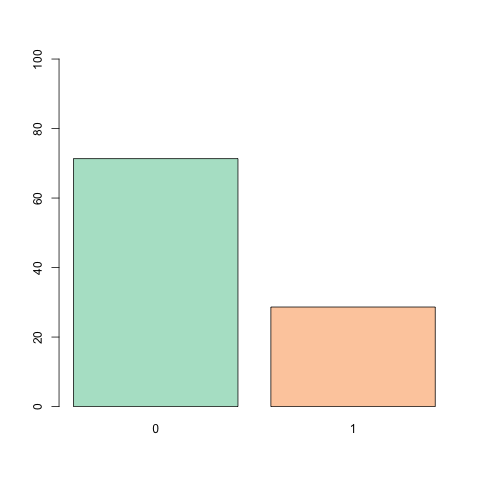
\includegraphics[width=0.8\textwidth]{ThesisTemplate/usingLatex/chapter4Images/figure4_6.png}
    \caption{Class Distribution of the liver dataset.\newline 0 represents the cases were the patient was not identified as a liver patient and 1 represents those cases were the patient was identified as a liver patient.}
    \label{fig:my_label}
\end{figure}

\subsubsection{Diabetes}
This dataset comprise 768 instances of health data from female Pima Indian patients of at least 21 years of age. There are 8 attributes and one target variable. The target variable indicates whether the individual will develop diabetes within 5 years (1) or not (0). The attributes were as follows:
\begin{itemize}
    \item Pregnancies indicates the number of times the patient pregnant
    \item GlucosePlasma indicates the glucose concentration at 2 hours in an oral glucose tolerance test
    \item BloodPressureDiastolic indicates the diastolic blood pressure (mm Hg)
    \item SkinThicknessTriceps indicates triceps skin fold thickness ( in mm)
    \item Insulin2-Hour indicates the serum insulin concentration  (mu U/ml)
    \item BMI indicates body mass index (weight in kg/(height in m \textsuperscript{2})
    \item DiabetesPedigreeFunctionDiabetes is a pedigree function calculated by the original authors of the study which takes family history of diabeted into account
    \item Age records the age of the patient (years)
\end{itemize}
 The dataset was used in a study looking at the ADAP algorithm and further details about the pedigree function and other variables can be found in the article \cite{Smith:1988wy}.
 
The exploratory data analysis carried out on this dataset is documented in the cited github repository as DiabetesEDA.R.\newline
The target label was already set to 0 (did not develop diabetes within 5 years) and 1 (did develop diabetes within 5 years), so no recoding of the data was necessary.\newline
A check for missing data revealed none, and Smith \textit{et al.,} indicate that they replaced any missing data with 0 (which does not always make sense, e.g. for blood pressure). No further modification of the dataset were necessary and the dataset was saved as csv file for later use.
The class distribution was compiled and presented as a graph (see figure 4.4).

\begin{figure}[H]
    \centering
    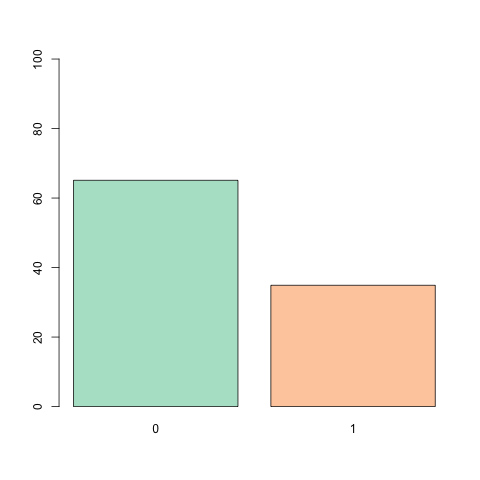
\includegraphics[width=0.8\textwidth]{ThesisTemplate/usingLatex/chapter4Images/figure4_8.png}
    \caption{Class Distribution of the diabetes dataset.\newline 0 represents the cases were the patient did not develop diabetes within 5 years and 1 represents the cases where the patient did develop diabetes within 5 years.}
    \label{fig:my_label}
\end{figure}

Compare this distribution with current incidence of the disease - could we randomly sample the data to mimic in the wild distribution????

\subsubsection{Lower Back Pain dataset}
% need citations
This dataset was originally built by Dr Henrique da Mota with a view to classify patient as one of 3 class: Normal, patients with disk hernia and patients with spondylolisthesis. In a second classifying task, the two types of sufferers were grouped as one abnormal category. This dataset was first uploaded to UCI (see http://archive.ics.uci.edu/ml/datasets/vertebral+column#) and then uploaded to Kaggle (see https://www.kaggle.com/sammy123/lower-back-pain-symptoms-dataset) as a binary classification task dataset (normal/abnormal).\newline
The dataset consists of 310 instances with 13 attributes (12 numeric predictors and 1 target label) as follows:
\begin{itemize}
    \item pelvic incidence
    \item pelvic tilt
    \item lumbar lordosis angle
    \item sacral slope
    \item pelvic radius
    \item degree spondylolisthesis
    \item pelvic slope
    \item Direct tilt
    \item thoracic slope
    \item cervical tilt
    \item sacrum angle
    \item scoliosis slope
\end{itemize}

The exploratory data analysis for this dataset is documented in the cited github repository as LowBackPainEDA.R.\newline
For ease of reading and  manipulation, the columns names were replaced by the actual name of the predictor (removing col x from the name) and the unused column X was removed.\newline
The target label was set as abnormal or normal so the data was recoded to be 1 for abnormal and 0 for normal, in line with the other datasets.
There were no missing values in the dataset.

\begin{figure}[H]
    \centering
    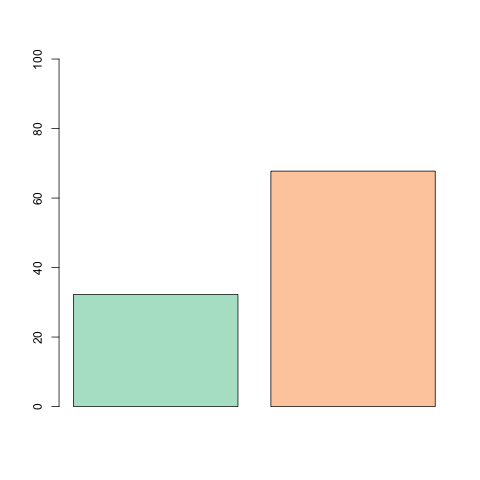
\includegraphics[width=0.8\textwidth]{ThesisTemplate/usingLatex/chapter4Images/figure4_12.png}
    \caption{Class Distribution of the low back pain dataset.\newline 0 represents the patients with normal spine, 1 identifies patients with abnormal spine (either disk hernia or spondylolisthesis }
    \label{fig:my_label}
\end{figure}

Uncharacteristically for a classification task, the abnormal class contains a higher number of instances than the normal class. This is unusual and in order to observe a class distribution more in line with those seen in other datasets in this project, random sampling of the dataset was  carried out so as to create a modified dataset with more normal samples than abnormal. To obtain the new dataset, 7\% of the abnormal instances were  retained (resulting in a higher prevalence than current estimates of 1-3\%) %citation needed here
and 100 \% of the normal instances were retained. Figure 4.6 shows the modified dataset class distribution.

\begin{figure}[H]
    \centering
    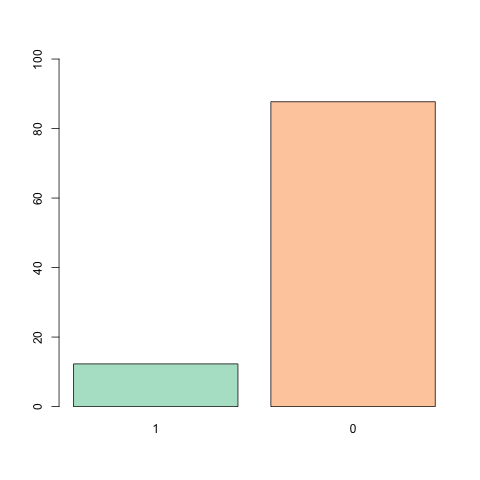
\includegraphics[width=0.8\textwidth]{ThesisTemplate/usingLatex/chapter4Images/figure4_14.png}
    \caption{Class Distribution of the modified low back pain dataset.\newline 0 represents the patients with normal spine, 1 identifies patients with abnormal spine (either disk hernia or spondylolisthesis }
    \label{fig:my_label}
\end{figure}


\subsubsection{Heart Attack Dataset}

This dataset is a subset from a multi centre, larger study which looked at patients with and without heart disease. The dataset was obtained from kaggle (see https://www.kaggle.com/imnikhilanand/heart-attack-prediction); the complete dataset appears to be available from UCI (see https://archive.ics.uci.edu/ml/datasets/heart+Disease) though some of the files may be corrupted and the classification tasks of the original datasets is not binary.
The original dataset was made up of 76 predictors but in this dataset this has been reduced to 13 and a target variable:
\begin{itemize}
    \item (age) 
    \item (sex) 
    \item (cp) 
    \item (trestbps) 
    \item (chol) 
    \item (fbs) 
    \item (restecg) 
    \item (thalach) 
    \item (exang) 
    \item (oldpeak) 
    \item (slope) 
    \item (ca) 
    \item (thal) 
\end{itemize}

The exploratory data analysis is documented in the cited github repository as HeartAttackEDA.R.\newline
Nine column contained missing values, and those were replaced with the mean value for that column. Examination of the data structure revealed that columns "chol" (for cholesterol value) and "thalach" (maximum heart rate achieved) were factors with more than 53 levels (the maximum that can be handled by Random Forest), 154 and 72 levels, respectively. The number of levels was reduced by grouping levels into categories:
\begin{table}[!htbp]
\centering
\caption{Grouping of levels for columns "chol" and "thalach" (Heart Disease Dataset)}
\begin{tabular}{*5c}
  \hline
  \multicolumn{2}{c}{Cholesterol} & \multicolumn{2}{c}{Thalach} \\
  \hline
  \hline
Level Value & New Level & Level Value & New Level\\ 
  \hline
    $<$100  & 100 & $\leq$90 & 90 \\ 
   $<$175 $\leq$150 & 175 & $>$90 $\leq$95   &  95 \\ 
  $<$200 $\geq$175 & 200 & $>$95 $\leq$100  & 100  \\ 
   $>$200 $\leq$225 & 225 & $>$100 $\leq$105 & 105  \\ 
   $>$225 $<$250  & 250 & $>$105 $\leq$110 & 110  \\ 
   $>$250 $<$275  & 275 & $>$110 $\leq$115 & 115  \\ 
   $>$275 $<$300  & 300 & $>$115 $\leq$120 & 120   \\ 
   $>$300 $<$325  & 325 & $>$120 $\leq$125 & 125   \\ 
   $>$325 $<$350  & 350 & $>$125 $\leq$130 & 130  \\ 
   $>$350 $<$375  & 375 & $>$130 $\leq$135 & 135  \\ 
   $>$375 $<$400  & 400 & $>$135 $\leq$140 & 140 \\ 
   $>$400 $<$425  & 425 & $>$140 $\leq$145 & 145\\ 
   $>$425 $<$450  & 450 & $>$145 $\leq$150 & 150\\ 
   $>$450 $<$475  & 475 & $>$150 $\leq$155 & 155\\ 
   $>$475 $<$500  & 500 & $>$155 $\leq$160 & 160\\ 
  `$>$500 $<$525  & 525 & $>$160 $\leq$165 & 165 \\ 
   $>$525 $<$550  & 550 & $>$165 $\leq$170 & 170 \\ 
   $>$550 $<$575  & 575 & $>$170 $\leq$175 & 175 \\ 
   $>$575 $<$600  & 600 & $>$175 $\leq$180 & 180 \\ 
                  &     & $>$180 $\leq$185 & 185 \\ 
                  &     & $>$185 $\leq$190 & 190 \\ 
   \hline
\end{tabular}
\end{table}

The target label was already set as either 0 (no heart disease) or 1 (heart disease) so this did not need to be modified. 
The class distribution was plotted (see Figure 4.7)

\begin{figure}[H]
    \centering
    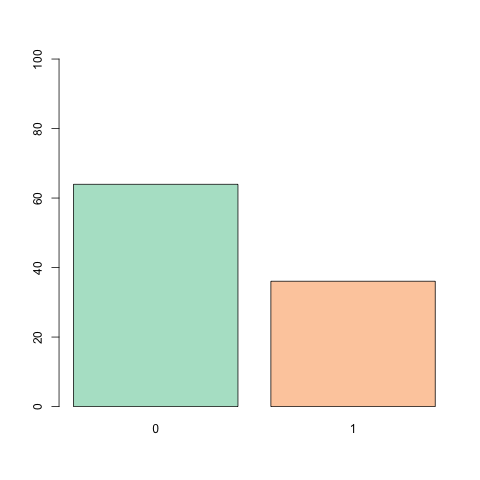
\includegraphics[width=0.8\textwidth]{ThesisTemplate/usingLatex/chapter4Images/figure4_16.png}
    \caption{Class Distribution of the heart disease dataset.\newline 0 represents the patients with no heart disease, 1 identifies patients with heart disease}
    \label{fig:my_label}
\end{figure}

This dataset is fairly balanced. In order to create a more imbalanced dataset, random sampling of the data which will retain all of the "normal" cases and only 10\% of the "positive" cases was carried out. The modified dataset was saved for future use in the project. The new class distribution is shown in figure 4.8 and reflects real-life prevalence of heart disease in the UK (6.7\% in men and 4.2\% in women)

\begin{figure}[H]
    \centering
    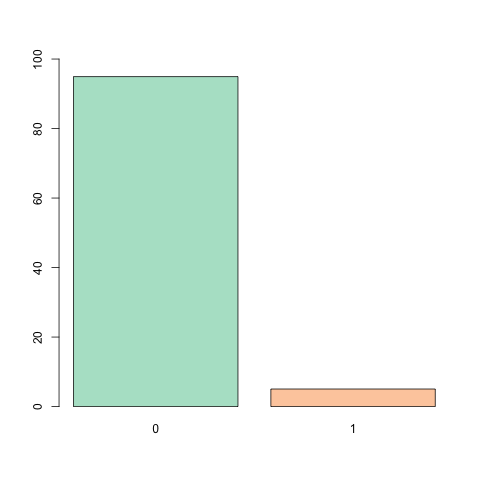
\includegraphics[width=0.8\textwidth]{ThesisTemplate/usingLatex/chapter4Images/figure4_18.png}
    \caption{Class Distribution of the heart disease dataset.\newline 0 represents the patients with no heart disease, 1 identifies patients with heart disease}
    \label{fig:my_label}
\end{figure}

\subsubsection{Autism dataset}




\subsubsection{Fertility dataset}

\subsection{Class distribution comparisons between datasets}


\begin{table}[H]
\centering
\begin{tabular}{lrr}
  \hline
Datasets & Majority.Class & Minority.Class \\ 
  \hline
Cervical\_Cancer & 95.45 & 4.55 \\ 
  Breast\_Cancer & 62.74 & 37.26 \\ 
  Liver\_Disease & 71.36 & 28.64 \\ 
  Diabetes & 65.10 & 34.90 \\ 
  Lower\_Back\_Pain & 67.74 & 32.26 \\ 
  Lower\_Back\_Pain modified & 87.72 & 12.28 \\ 
  Heart\_Attack & 63.95 & 36.05 \\ 
  Heart\_Attack modified & 94.95 & 5.05 \\ 
  Autism & 73.15 & 26.85 \\ 
  Fertility & 88.00 & 12.00 \\ 
   \hline
\end{tabular}
\end{table}

\begin{figure}[H]
    \centering
    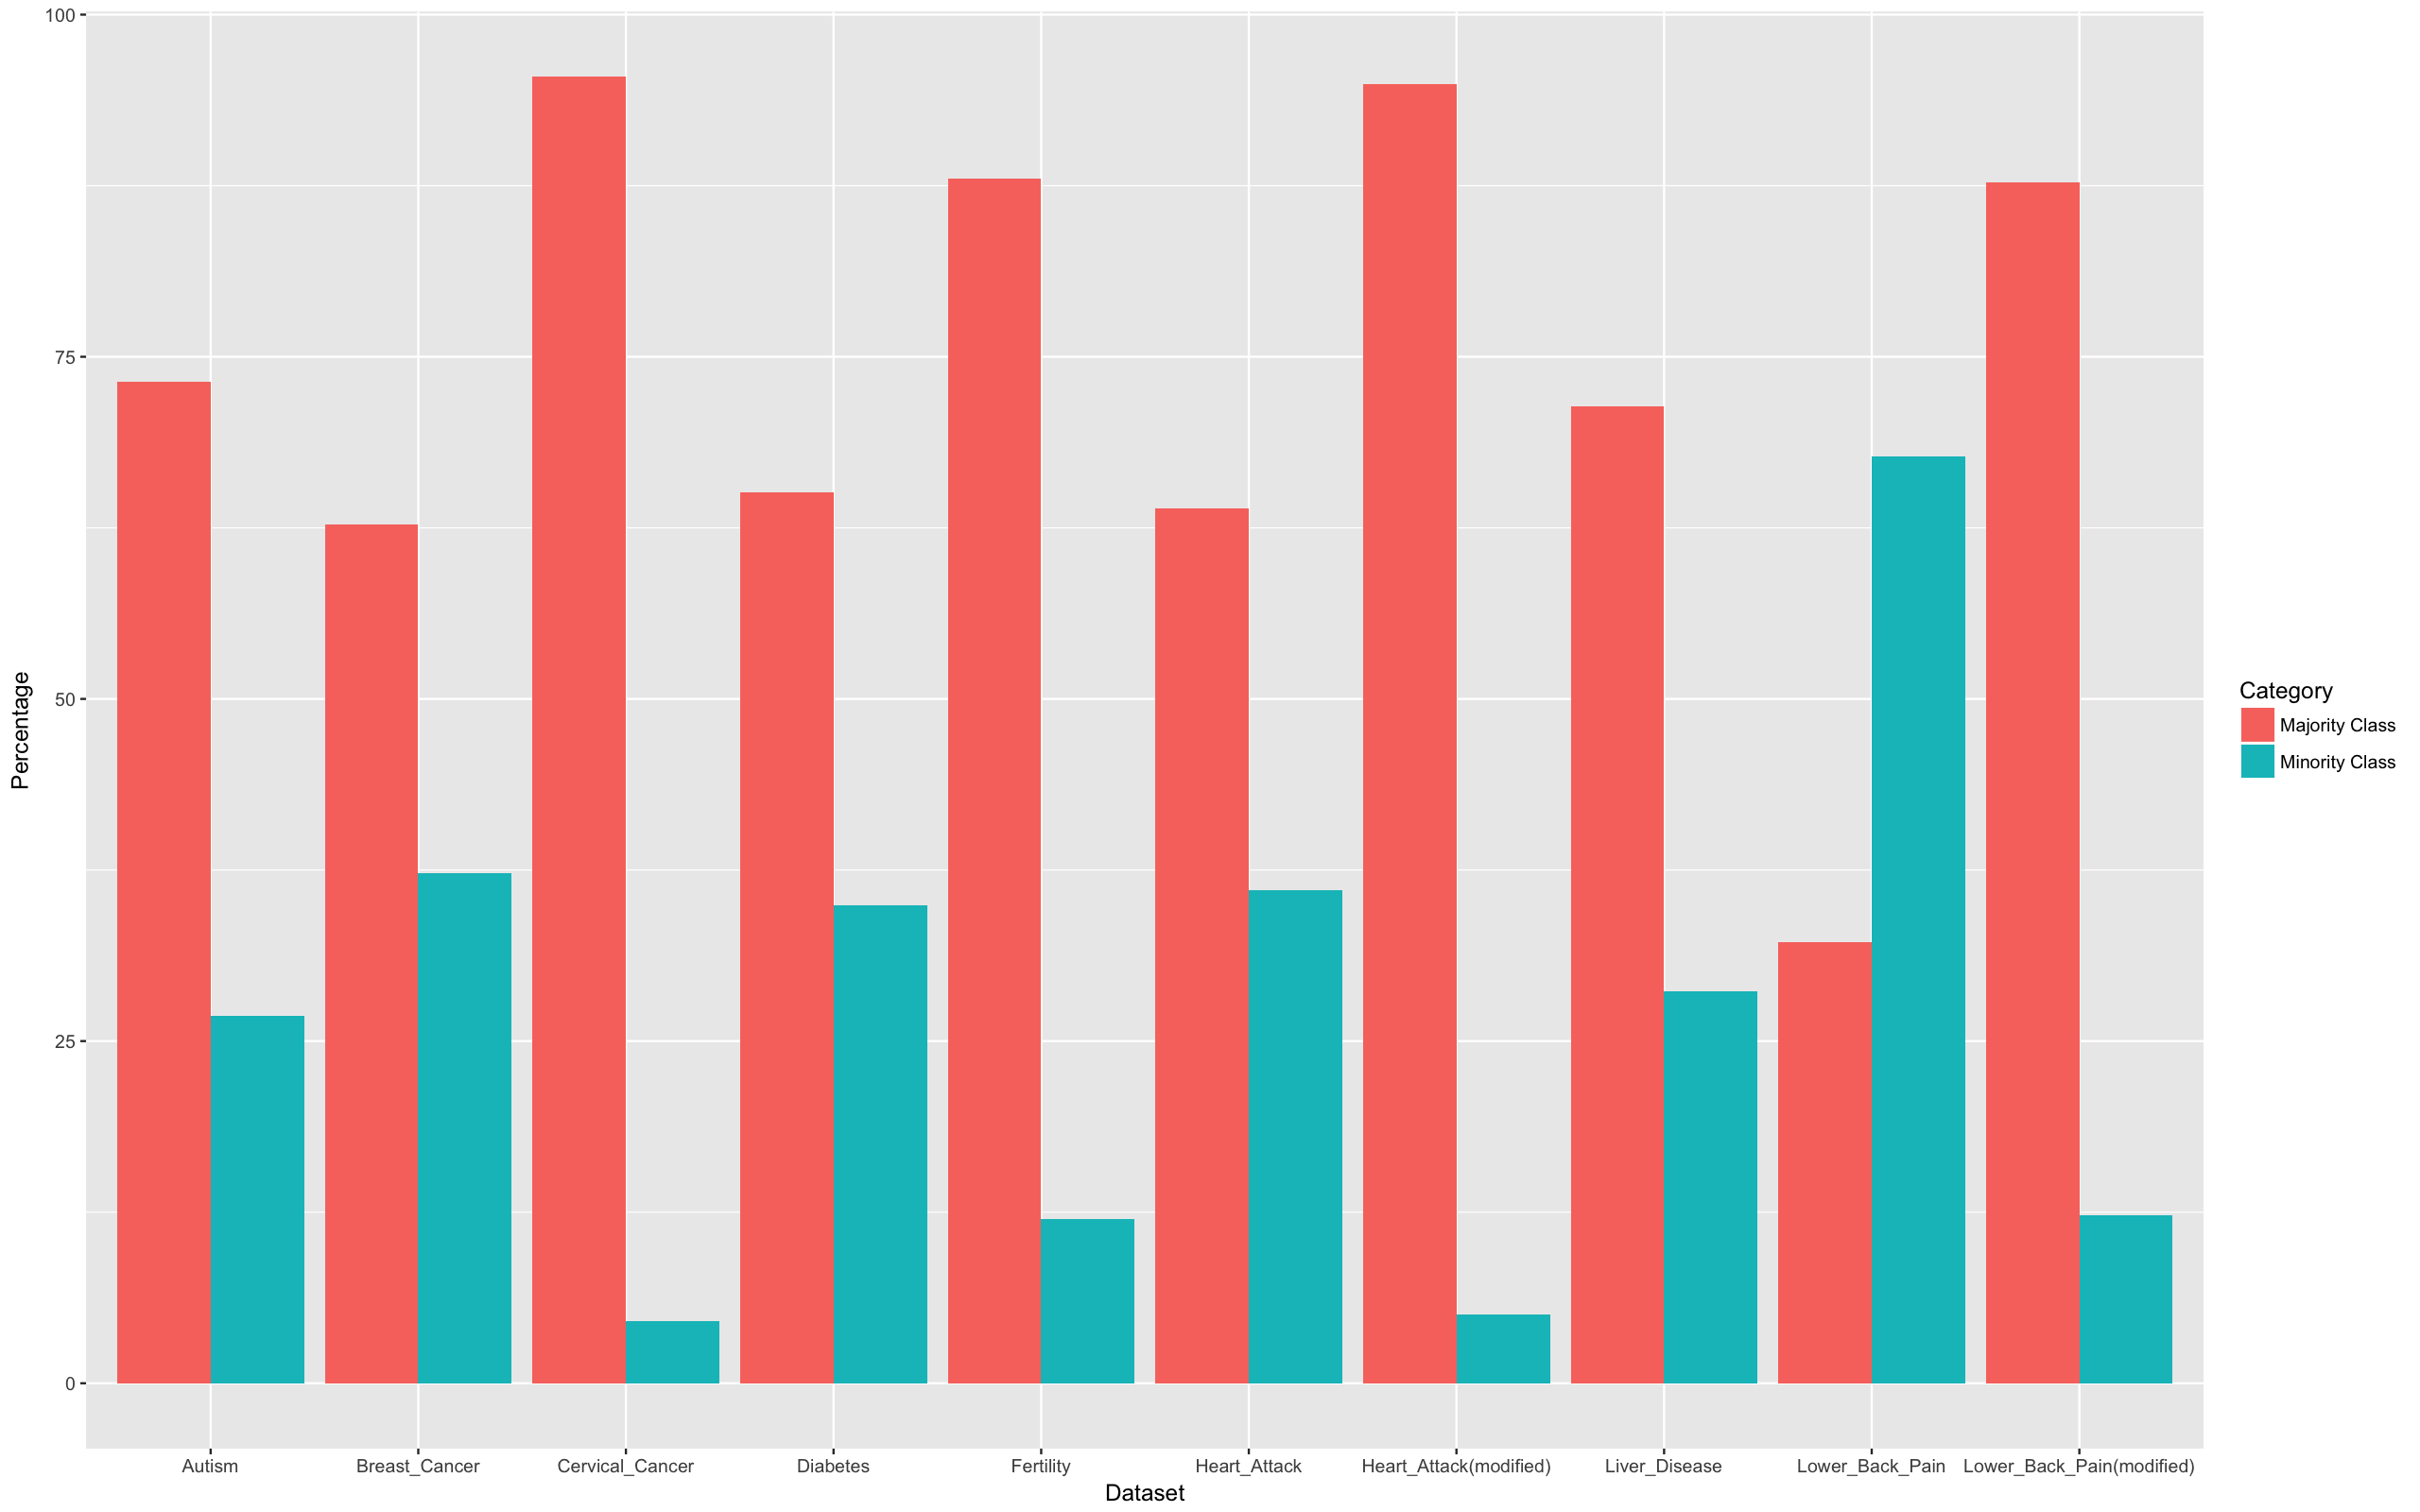
\includegraphics[width=0.8\textwidth]{ThesisTemplate/usingLatex/chapter4Images/figure4_1b.png}
    \caption{Class Distribution of the chosen datasets.\newline In all cases the majority class is the class representing healthy subjects and the minority class is the class representing affected subjects. In the case of the lower back pain dataset, the class representing the "abnormal" patients counts more instances than the the class representing the "normal" patients, however the terms minority and majority were kept for consistency with the other datasets.}
    \label{fig:my_label}
\end{figure}
\section{Modelling the datasets}
\subsection{Random Forest}
Random forest was used with all the datasets. An R script (see linked repository, Experiment1.R and RandomForestModelling.R) was created to classify all 10 datasets and obtain a baseline of the performance that could be obtained on the mostly untouched data.
The dataset were uploaded as a list which was iterated through by the R function randomForest. The data split was 70:30 train: test and the number of trees was 1000, proximity and importance were both set as true.\newline
The RandomForestModelling.R script allowed for a data frame to be created to contain performance metrics of the algorithm for each dataset.\newline
The performance metrics used were Accuracy, sensitivity, precision and F1 score.\newline

\subsection{Support Machine Vector}
\subsection{K-Nearest Neighbour}
\subsection{Naive  Bayes}
\section{Modelling the datasets with data-level solutions applied}
\subsection{Undersampling of the majority class}
\subsubsection{Undersampling majority class: 40\%}
An R script was created to fit Random Forest to the datasets after under sampling the majority class in an attempt to address the class imbalance. This will lead to loss of data and though we expect some metrics to improve it is likely that others will also worsen.\newline
A function to choose the proportion of each class to include in the experiment was devised and several different percentages of majority class data were tested, while always retained 100 \% of the minority class.  The default value for the function was 40\% of the majority class and 100\% of the minority class retained. The same experiment was also carried out for 60\% of majority class and 75\% of majority class.\newline
\subsubsection{Undersampling majority class: 60\%}
In each case the accuracy, sensitivity precision and F1 score were recorded.\newline

\subsubsection{Undersampling majority class: 60\%}

\subsection{Oversampling of the minority class}
Experiment 3 Oversampling of the minority class
This time, in order to address the class imbalance, the SMOTE function was applied to the datasets. SMOTE (Synthetic Minority Oversampling Technique) is a technique devised in 2002 (citation). A smote()  R function exists in package DMwR and was used for these experiments.\newline
%Here detail the smote function
The k value is set by default at k=5. This value needs to be set to 3 or 4 for the modified heart attack dataset since there so few observations in the training sets after the data has been split. if k exceeds the number of minority class observations in the training set, an error will occur as there will not be enough points to create the new data point.\newline
The smote() function is applied only to the training set, not the testing set.\newline

The parameters used when applying smote to the non modified datasets were  k=4


The smote() function was applied to the modified heart attack dataset and low back pain dataset with separate parameters from the other datasets, as the generally lower number of observation existing in the sample meant that too few majority class observations were retained. The parameters for these datasets were 200, 600 and k= 4.
Finally the fertility datasets consists of a low number of observation and smote() was also applied with separate parameters so as to retain a larger number of majority class observation (200, 600 k=4) % check those numbers.




 



\subsection{k-mean}


\section{Modelling the datasets with algorithm-level solutions applied}

\section{Conclusions}

The main conclusions for this chapter.


